\documentclass[t,aspectratio=169]{beamer}
\usetheme[progressbar=frametitle]{metropolis}
\usefonttheme{professionalfonts}
\usepackage{appendixnumberbeamer}

\usepackage{booktabs}
\usepackage[scale=2]{ccicons}

\usepackage{graphics,graphicx,amssymb,amsmath,pgf,comment,hyperref}
%\usepackage[xcolor=pst]{pstricks}
\usepackage{array}
\usepackage{pgfshade}
\usepackage[round]{natbib}
\usepackage[absolute,overlay]{textpos}
\usepackage{pifont}
\usepackage{dcolumn}
\usepackage{textpos}
\usepackage{color}					
\usepackage{xcolor,colortbl}
\usepackage{tikz}
\usepackage{bbm}
\usepackage{curves}
\usepackage{mathtools}
\usepackage{times}
\usepackage{verbatim}
\usetikzlibrary{snakes,arrows,shapes,positioning}
\def\augie{\fontencoding{T1}\fontfamily{augie}\selectfont}

\usepackage{pgfplots}
\usepgfplotslibrary{dateplot}
\usepackage{bm}

\usepackage{xspace}
\newcommand{\themename}{\textbf{\textsc{metropolis}}\xspace}

\definecolor{beamcol}{RGB}{5,48,97}
\definecolor{beamcol2}{RGB}{33,102,172}
\usecolortheme[named=beamcol]{structure}

\setbeamertemplate{caption}{\raggedright\insertcaption\par}
\usetikzlibrary{calc,decorations.pathmorphing,patterns}
\pgfdeclaredecoration{penciline}{initial}{
    \state{initial}[width=+\pgfdecoratedinputsegmentremainingdistance,
    auto corner on length=1mm,]{
        \pgfpathcurveto%
        {% From
            \pgfqpoint{\pgfdecoratedinputsegmentremainingdistance}
                      {\pgfdecorationsegmentamplitude}
        }
        {%  Control 1
        \pgfmathrand
        \pgfpointadd{\pgfqpoint{\pgfdecoratedinputsegmentremainingdistance}{0pt}}
                    {\pgfqpoint{-\pgfdecorationsegmentaspect
                     \pgfdecoratedinputsegmentremainingdistance}%
                               {\pgfmathresult\pgfdecorationsegmentamplitude}
                    }
        }
        {%TO
        \pgfpointadd{\pgfpointdecoratedinputsegmentlast}{\pgfpoint{1pt}{1pt}}
        }
    }
    \state{final}{}
}


\title{Owning the Agent: Hospital Influence on Physician Behaviors}
\date{}
\author{Haizhen Lin \& \textbf{Ian McCarthy} \& Michael Richards}
\institute{January 4, 2020}

\begin{document}
\maketitle

\section{Motivation}

\begin{frame}[t]{Hospital in Physician Agency Problem}
\bigskip
    \begin{tikzpicture}
    % draw horizontal line
    \draw[thick, -] (1cm,0) -- (10cm,0);

    % draw node
    \draw[ultra thick] (1,0) node[left=3pt,thick] {Physician};
    \draw[ultra thick] (10,0) node[right=3pt,thick] {Patient};

    \only<2-3>{
        % draw and label vertical lines
        \draw[thick, -] (4 cm,7pt) -- (4 cm,-7pt);
        \draw[thick, -] (7 cm,7pt) -- (7 cm,-7pt);
        \draw[thick] (7, -1) node(Pat)[above=1pt] {$y_{1}$};
        \draw[thick] (4, -1) node(Phy)[above=1pt] {$y_{2}$};
    }

    \only<3>{
        \draw[ultra thick] (7,-3) node(ur)[above=3pt,thick] {Hospital};
        \draw [beamcol, thick, ->] (ur) [in = 270] to [out = 60]  (Pat);
        \draw [beamcol, thick, ->] (ur) [in = 270] to [out = 120]  (Phy);
    }

    \only<4-6>{
        \draw[thick, -] (5 cm,6pt) -- (5 cm,-6pt);
        \draw[thick] (5, -1) node(Pat)[above=1pt] {$y^{*}$};
    }

    \only<5-6>{
        \draw[ultra thick] (0,-0.4) node[thick] {\& Hospital};
    }

    \only<6>{
        \draw[thick, ->] (4.8, -1) -- (3.2,-1);
        \draw[thick, -] (3 cm,6pt) -- (3 cm,-6pt);
        \draw[thick] (3, -1) node(Phy)[above=1pt] {$y^{*}_{h}$};
    }
    \end{tikzpicture}

\end{frame}

\tikzstyle{every picture}+=[remember picture]
\everymath{\displaystyle}
\begin{frame}{Changing Physician Relationships}
    \begin{figure}
        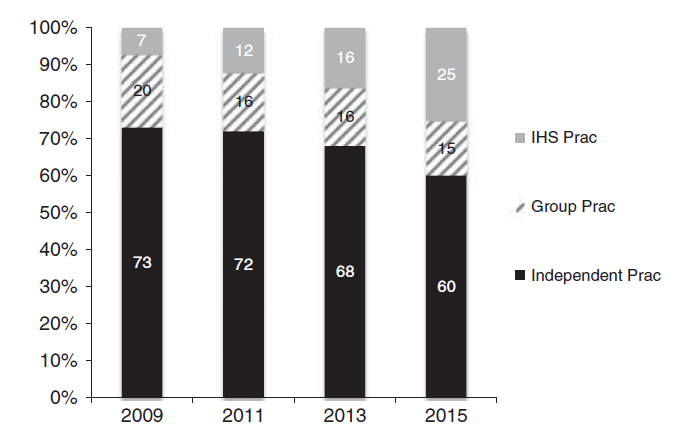
\includegraphics[height=2.4in,keepaspectratio]{Richardsetal.png}
        \caption{Richards \textit{et al.}, Medical Care, 2016}
    \end{figure}
\end{frame}

\begin{frame}{In context}
    \begin{itemize}
        \item Physician agency (Clemens \& Gottlieb 2014, AER; Afendulis \& Kessler 2007, AER; Gruber \& Owings 1996, RAND; Iizuka 2012, AER)
        \item Supply-side variation (Finkelstein \textit{et al.} 2016, QJE; Molitor 2018, AEJ: Policy)
        \item Vertical integration (Cuellar \& Gertler 2006, JHE; Ciliberto \& Dranove 2006, JHE; Baker \textit{et al.} 2016, JHE; Koch \textit{et al.} 2017, JHE)
    \end{itemize}
\end{frame}

\section{Estimation Strategy}
\begin{frame}{Estimation Strategy}
    \tikzstyle{na} = [baseline=-.5ex]
    \only<1->{
        Observed care at time $t$ is
        \begin{equation*}
            y_{ijk} =
            \tikz[baseline]{
                \node[fill=blue!20,anchor=base] (t1)
                {$ \alpha_{i} + x_{i}\beta $};
            } +
            \tikz[baseline]{
                \node[fill=red!20, ellipse, anchor=base] (t2)
                {$\Gamma_{jk}$};
            } + \epsilon_{ijk}
        \end{equation*}
        \begin{itemize}[<+-| alert@+>]
            \item[]<2-> Patient Preferences
                \tikz[na] \node[coordinate] (n1) {};
            \item[]<3-> Physician and hospital characteristics
                \tikz[na] \node[coordinate] (n2) {};
        \end{itemize}

        \begin{tikzpicture}[overlay]
            \path[->]<2-> (n1) edge [bend right] (t1);
            \path[->]<3-> (n2) edge [out=0, in=-90] (t2);
        \end{tikzpicture}
    }
\end{frame}



\section{Data}
\begin{frame}{Data Sources}
    \begin{itemize}
        \item<1-> CMS: 100\% inpatient and institutional outpatient Medicare claims data (2008-2015)
        \item<1-> SK\&A: Hospital ownership of physician practices and practice characteristics
        \item<2-> AHA, HCRIS, POS: Hospital characteristics
        \item<2-> Annual IPPS Impact Files: Hospital cost-to-charge ratios (CCR)
        \item<2-> ACS: County-level demographics, education, income, and employment
    \end{itemize}
\end{frame}

\begin{frame}{Data Structure}
    \begin{itemize}
        \item<1-> Measure annual spending per patient for each physician/hospital pair
        \item<1-> Planned inpatient stays (elective admissions initiated by a physician, clinic, or HMO referral) and outpatient operations
    \end{itemize}
  \uncover<2->{ $\longrightarrow$ 518,398 unique observations at the physician/hospital/year \\
   $\longrightarrow$ 7.5mm inpatient stays (47\% of total) and 24mm outpatient procedures}
\end{frame}

\section{Vertical Integration and Treatment Intensity}
\begin{frame}{Estimated Effects of Vertical Integration}
    \only<1>{
    Two-step estimation strategy:
    \begin{enumerate}
        \item Estimate $y_{ijk} = \alpha_{i} + x_{i}\beta + \Gamma_{jk} + \epsilon_{ijk}$ at patient level (separately by year)
        \item Estimate $\hat{\Gamma}_{jkt} = \gamma_{j} + \gamma_{k} + \tau_{t} + z_{jkt}\delta + \eta_{jkt}$ with physician-hospital panel
    \end{enumerate}
    }
    \only<2->{
    \begin{equation*}
        \hat{\Gamma}_{jkt} = \gamma_{j} + \gamma_{k} + \tau_{t} + z_{jkt}\delta + \eta_{jkt},
    \end{equation*}
    }
    \only<3->{
        \begin{table}[htb!]
        \centering
        \centerline{
        \begin{tabular}{l|rr}
            Outcome & Estimate & St. Error \\
            \hline\hline \onslide<4->{\vspace{-.1in}\\
            Total Medicare Payments & 76.176** & (30.911)  \onslide<5->{\\
            Total Hospital Costs & 133.063***  & (42.099) \onslide<6->{\\
            Total Procedures   &   0.014***  &  (0.004) }}}\\
            \hline
            \multicolumn{3}{l}{\footnotesize * p-value $<$0.1, ** p-value $<$0.05, *** p-value $<$0.01}
        \end{tabular}}
        \end{table}
    }
\end{frame}


\begin{frame}{Threats to Identification and Interpretation}
At least three concerns to interpret as effect on treatment intensity:
    \begin{enumerate}
        \item Standard issues with two-way FE estimator and time-varying treatment
        \item Reallocation from other OP facilities (without matching hospital NPI)
        \item Moving from clinic (unobserved) to OP facility
    \end{enumerate}
\end{frame}


\section{Event Studies}
\begin{frame}{Total Medicare Payments}
    \begin{figure}
        \centering
        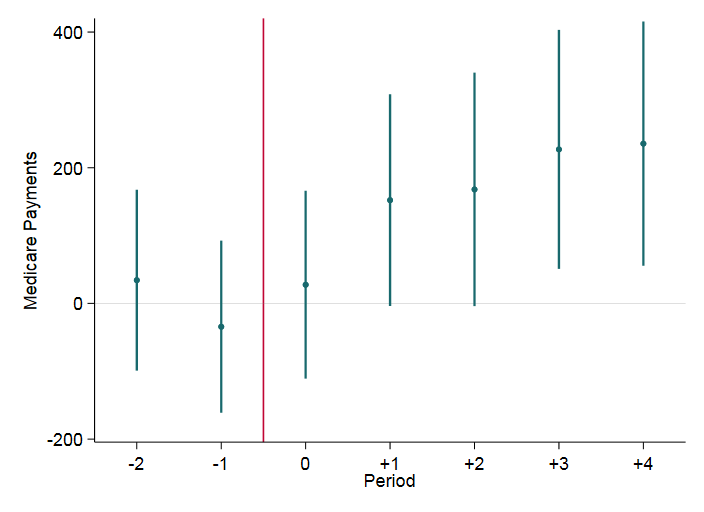
\includegraphics[height=2.5in,width=5in,keepaspectratio]{EventPay_All_2011}
    \end{figure}
\end{frame}

\begin{frame}{Total Hospital (IP \& OP) Costs}
    \begin{figure}
        \centering
        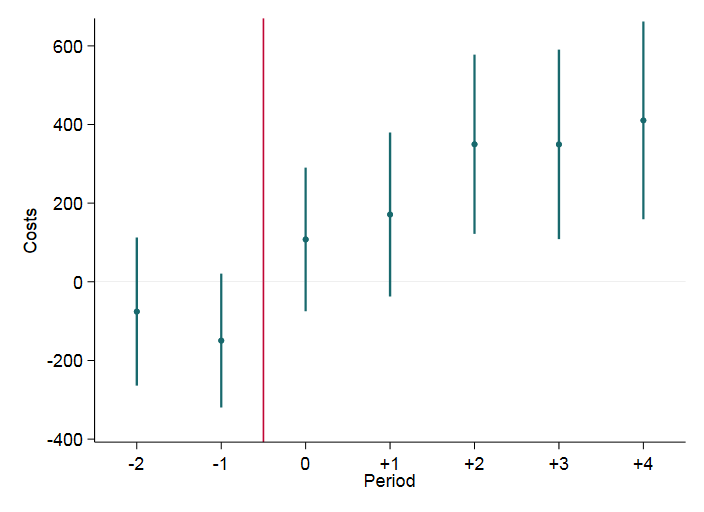
\includegraphics[height=2.5in,width=5in,keepaspectratio]{EventCharge_All_2011}
    \end{figure}
\end{frame}

\begin{frame}{Takeaways}
    \begin{itemize}
        \item Increase in payments and costs
        \item Evidence consistent with common trends assumption for total payments and costs
        \item Concerns about limited pre-period data
    \end{itemize}
\end{frame}


\section{Treatment Intensity vs Reallocation}
\begin{frame}{Want to isolate treatment intensity effect}
    \begin{enumerate}
        \item Focus on patients with no change in physician/hospital pairs over time
        \item Examine outcomes within an inpatient stay
    \end{enumerate}
\end{frame}

\begin{frame}{Aggregate Outcomes without Reallocation}
    \vspace{0.75in}
    \begin{table}[htb!]
    \centering
    \centerline{
    \begin{tabular}{l|rr}
        Outcome & Estimate & St. Error \\
        \hline\hline \onslide<2->{\vspace{-.1in}\\
        Total Medicare Payments & 64.134** & (30.858)  \onslide<3->{\\
        Total Hospital Costs & 122.894***  & (42.130) \onslide<4->{\\
        Total Procedures & 0.013** & (0.004) }}}\\
        \hline
        \multicolumn{3}{l}{\footnotesize * p-value $<$0.1, ** p-value $<$0.05, *** p-value $<$0.01}
    \end{tabular}}
    \end{table}
\end{frame}

\begin{frame}{Effects on Components of Inpatient Stay}
    \vspace{0.5in}
    \begin{table}[htb!]
    \centering
    \centerline{
    \begin{tabular}{l|rr}
        Outcome & Estimate & St. Error \\
        \hline\hline
        Charges for: & & \\
        \hspace{.1in} Total Inpatient & 180.997*** & (49.771) \\
        \hspace{.1in} Medical Supplies & 40.564 & (30.024) \\
        \hspace{.1in} Operating Room & -11.029 & (22.928) \\
        \hspace{.1in} Anesthesia & 5.278 & (4.999) \\
        \hspace{.1in} Labs & 9.286 & (8.826) \\
        \hspace{.1in} Radiology & -5.943 & (6.058) \\
        \hspace{.1in} MRI & -0.514 & (1.359) \\
        \hline
        \multicolumn{3}{l}{\footnotesize * p-value $<$0.1, ** p-value $<$0.05, *** p-value $<$0.01}
    \end{tabular}}
    \end{table}
\end{frame}

\begin{frame}{Effects on Components of Inpatient Stay}
    \vspace{0.5in}
    \begin{table}[htb!]
    \centering
    \centerline{
    \begin{tabular}{l|rr}
        Outcome & Estimate & St. Error \\
        \hline\hline
        Counts of: & & \\
        \hspace{.1in} ICU Days  & 0.021  & (0.013) \\
        \hspace{.1in} Procedures  & 0.030*** & (0.009) \\
        \hline
        Medicare payments: & 338.846** & (138.981) \\
        \hline
        \multicolumn{3}{l}{\footnotesize * p-value $<$0.1, ** p-value $<$0.05, *** p-value $<$0.01}
    \end{tabular}}
    \end{table}
\end{frame}

\section{Heterogeneous Effects}
\begin{frame}{Unconditional Quantile Results: Payments}
    \begin{figure}
        \centering
        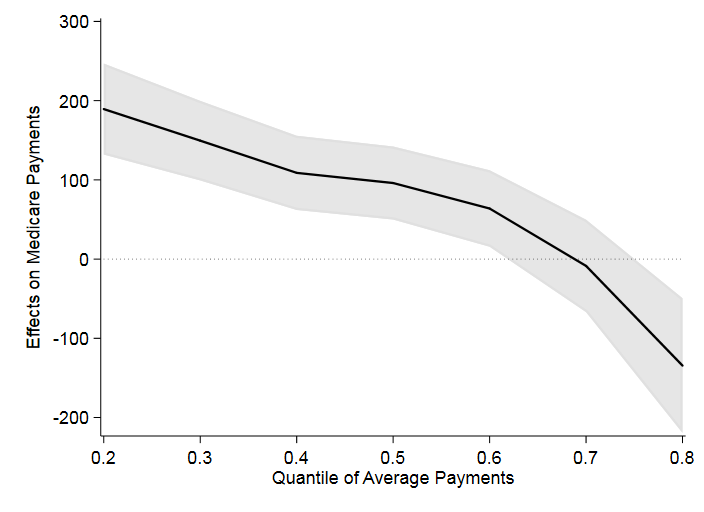
\includegraphics[height=2.5in,width=5in,keepaspectratio]{QReg_Payment}
    \end{figure}
\end{frame}

\begin{frame}{Unconditional Quantile Results: Hospital Costs}
    \begin{figure}
        \centering
        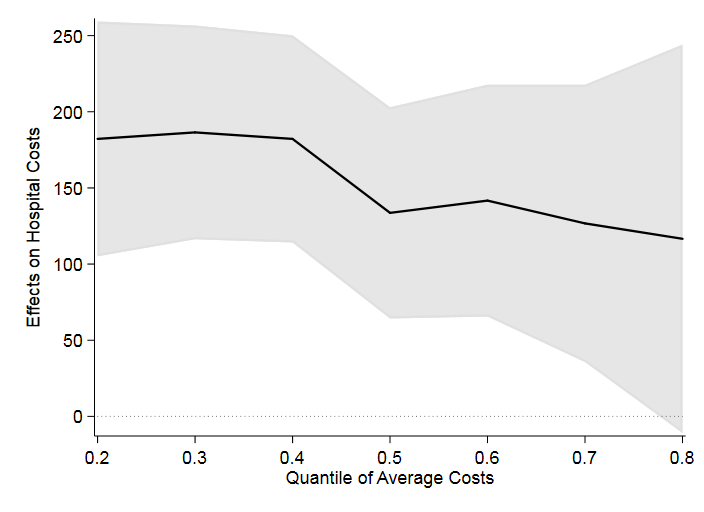
\includegraphics[height=2.5in,width=5in,keepaspectratio]{QReg_Charge}
    \end{figure}
\end{frame}

\begin{frame}{Unconditional Quantile Results: Procedures}
    \begin{figure}
        \centering
        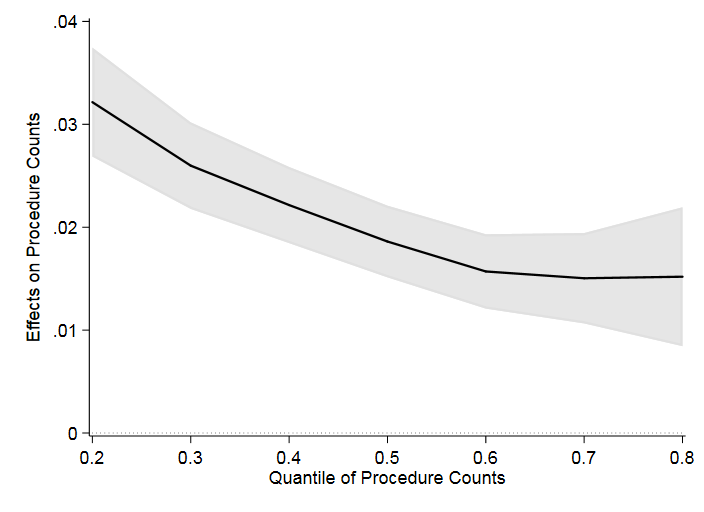
\includegraphics[height=2.5in,width=5in,keepaspectratio]{QReg_Procs}
    \end{figure}
\end{frame}


\section{Main Takeaways}
\begin{frame}{Summary of Results}
    \only<1>{
        \metroset{block=fill}
        \begin{block}{Overall Results}
            \begin{itemize}
                \item Increase in Medicare payments (\$75-\$200) and hospital costs (\$130-\$350)
                \item Extrapolates to between \$55mm and \$146mm in additional Medicare payments per year
                \item 4-10\% of within-physician variation across hospitals explained by vertical integration
            \end{itemize}
        \end{block}
    }

\end{frame}

\section*{Thank You}


\end{document}






